\documentclass[aps,prb,twocolumn,superscriptaddress,footinbib,amsmath,amssymb,floatfix]{revtex4}
\usepackage[dvips]{epsfig}
\usepackage{graphicx}
\usepackage{ifthen}
\usepackage{dcolumn}% Align table columns on decimal point
\usepackage{bm}% bold math
\usepackage{multirow}
\usepackage{booktabs}
\usepackage{bm}% bold math
\usepackage{amsbsy}
\usepackage{amsmath}
\usepackage{amssymb}
\usepackage{subfigure}
\usepackage{wrapfig}

%Definition of new commands
\newcommand{\f}[2]{\ensuremath{\frac{\displaystyle{#1}}{\displaystyle{#2}}}}
\newcommand{\lr}[1]{\langle{#1}\rangle}
\newcommand{\colv}[2] {\left(\begin{array}{c} #1 \\ #2 \end{array}\right)}
\renewcommand{\thefootnote}{\fnsymbol{footnote}}
\newcommand{\be} {\begin{eqnarray}}
\newcommand{\ee} {\end{eqnarray}}
%--------------------------------------------------------------------------
%EQ COMMANDS
%--------------------------------------------------------------------------
\newcommand{\two}{\mspace{-2.0mu}}
\newcommand{\four}{\mspace{-4.0mu}}
\newcommand{\plus}{\mspace{-4.5mu}+\mspace{-3.5mu}}
\newcommand{\minus}{\mspace{-4.5mu}-\mspace{-3.5mu}}
\newcommand{\pp}{'\mspace{-2.0mu}'}
\newcommand{\xlb}[4]{#1\ifthenelse{\equal{#2}{0}}{}{_{\alpha #2}}
\mspace{-2.0mu}\genfrac{(}{)}{0pt}{1}{\ifthenelse{\equal{#3}{0}}{0}{l #3}} 
{\ifthenelse{\equal{#4}{0}}{0}{b #4}}}

\newcommand{\xkv}[4]{#1\mspace{-5.0mu}\left(\mspace{-8.0mu}
\begin{smallmatrix}#2\four{}\four{}\mspace{-8.0mu}&\pmb{\kappa}#3\\&\nu 
#4\end{smallmatrix}\mspace{-5.0mu}\right)}

\newcommand{\evect}[6]{#1\mspace{-4.0mu}\left(\mspace{-8.0mu}
\begin{smallmatrix}#2\mspace{-8.0mu}&\pmb{\kappa} #3 &b #5\\&\nu #4 &
\alpha #6\end{smallmatrix}\mspace{-5.0mu}\right)}

\newcommand{\varmat}[8]{\mspace{-5.0mu}\left(\mspace{-8.0mu}
\begin{smallmatrix}\ifthenelse{\equal{#3}{0}}{\mspace{-8.0mu}&b_{#1}&b_{#2}
\\&\alpha_{#1}&\alpha_{#2}} {\ifthenelse{\equal{#7}{0}}{#1\mspace{-8.0mu}&
\pmb{\kappa}#2#3\mspace{-8.0mu}&\pmb{\kappa}#4#5\mspace{-8.0mu}&\pmb{\kappa}
#6\\&\nu#2&\nu#4&\nu#6} {#1\mspace{-8.0mu}&\pmb{\kappa}#2#3\mspace{-8.0mu}&
\pmb{\kappa}#4#5\mspace{-8.0mu}&\pmb{\kappa}#6#7\mspace{-8.0mu}&\pmb{\kappa}
#8\\&\nu#2&\nu#4&\nu#6&\nu#8}}\end{smallmatrix}\mspace{-5.0mu}\right)}

\newcommand{\EXP}[1]{\exp\mspace{-5.0mu}\left[#1\right]\mspace{-3.0mu}}

\newcommand{\tpp}[2]{\left(\mspace{-2.0mu}\xkv{\omega}{}{}{}#1\xkv{\omega}
{}{'}{'}#2\xkv{\omega}{}{\pp}{\pp}\mspace{-2.0mu}\right)}



%--------------------------------------------------------------------------
\newcommand{\SUM}[2]{\ifthenelse{\equal{#1}{0}}{\sum_{
\alpha_{#2},b_{#2},l_{#2}}^{3,n,N}} {\ifthenelse{\equal{#1}{1}}{\sum_{
\alpha_{#2},b_{#2}}^{3,n}}{\sum_{\pmb{\kappa}#2,\nu#2}^{N,3n}}}}

\newcommand{\SUMprime}[2]{\ifthenelse{\equal{#1}{0}}
{\sum_{\alpha_{#2},b_{#2},l_{#2}}^{3,n,N}} 
{\ifthenelse{\equal{#1}{1}}{\sum_{\alpha_{#2},b_{#2}}^{3,n}}
{\sum_{\pmb{\kappa}^{'}#2,\nu#2}^{N,3n}}}}

\newcommand{\SUMalpha}[2]{\ifthenelse{\equal{#1}{0}}
{\sum_{\alpha_{#2}}^{3}} {\ifthenelse{\equal{#1}{1}}
{\sum_{\alpha_{#2},b_{#2}}^{3,n}}{\sum_{\pmb{\kappa}#2,\nu#2}^{N,3n}}}}
%--------------------------------------------------------------------------
\newcommand{\SUMalphap}[2]{\ifthenelse{\equal{#1}{0}}
{\sum_{\alpha'_{#2}}^{3}} {\ifthenelse{\equal{#1}{1}}
{\sum_{\alpha'_{#2},b'_{#2}}^{3,n}}{\sum_{\pmb{\kappa}#2,\nu#2}^{N,3n}}}}

\newcommand{\SUMb}[2]{\ifthenelse{\equal{#1}{0}}{\sum_{b_{#2}}^{n}}
 {\ifthenelse{\equal{#1}{1}}{\sum_{\alpha_{#2},b_{#2}}^{3,n}}
{\sum_{\pmb{\kappa}#2,\nu#2}^{N,3n}}}}

\newcommand{\SUMbp}[2]{\ifthenelse{\equal{#1}{0}}{\sum_{b'_{#2}}^{n}}
 {\ifthenelse{\equal{#1}{1}}{\sum_{\alpha'_{#2},b'_{#2}}^{3,n}}
{\sum_{\pmb{\kappa}#2,\nu#2}^{N,3n}}}}

\newcommand{\SUMl}[2]{\ifthenelse{\equal{#1}{0}}{\sum_{l_{#2}}^{N}}
 {\ifthenelse{\equal{#1}{1}}{\sum_{\alpha_{#2},b_{#2}}^{3,n}}
{\sum_{\pmb{\kappa}#2,\nu#2}^{N,3n}}}}

\newcommand{\SUMlp}[2]{\ifthenelse{\equal{#1}{0}}{\sum_{l'_{#2}}^{N}}
 {\ifthenelse{\equal{#1}{1}}{\sum_{\alpha'_{#2},b'_{#2}}^{3,n}}
{\sum_{\pmb{\kappa}#2,\nu#2}^{N,3n}}}}

\newcommand{\abcdt}[5]{\mspace{-4.0mu}\left(\mspace{-8.0mu}
\begin{smallmatrix}&\ifthenelse{\equal{#1}{}}{a}{#1}&\ifthenelse
{\equal{#3}{}}{c}{#3}\\&\ifthenelse{\equal{#2}{}}{b}{#2}&\ifthenelse
{\equal{#4}{}}{d}{#4}\end{smallmatrix}\mspace{-2.0mu};\ifthenelse
{\equal{#5}{}}{t}{#5}\right)}

\newcommand{\abcd}[4]{\mspace{-4.0mu}\left(\mspace{-8.0mu}
\begin{smallmatrix}&\ifthenelse{\equal{#1}{}}{a}{#1}&\ifthenelse
{\equal{#3}{}}{c}{#3}\\&\ifthenelse{\equal{#2}{}}{b}{#2}&\ifthenelse
{\equal{#4}{}}{d}{#4}\end{smallmatrix}\mspace{-3.0mu}\right)}

\newcommand{\abt}[3]{\mspace{-4.0mu}\left(\mspace{-8.0mu}\begin
{smallmatrix}&\ifthenelse{\equal{#1}{}}{a}{#1} \\&\ifthenelse{
\equal{#2}{}}{b}{#2}\end{smallmatrix}\mspace{-2.0mu};
\ifthenelse{\equal{#3}{}}{t}{#3}\right)}

\newcommand{\ab}[2]{\mspace{-4.0mu}\left(\mspace{-8.0mu}
\begin{smallmatrix}&\ifthenelse{\equal{#1}{}}{a}{#1} \\&\ifthenelse
{\equal{#2}{}}{b}{#2}\end{smallmatrix}\mspace{-3.0mu}\right)}

\newcommand{\kvbat}{\mspace{-4.0mu}\left(\mspace{-8.0mu}
\begin{smallmatrix} &\pmb{\kappa} &b \\ &\nu &\alpha\end{smallmatrix}
\mspace{-2.0mu};t\right)}
%--------------------------------------------------------------------------
\newcommand{\kvbatp}{\mspace{-4.0mu}\left(\mspace{-8.0mu}
\begin{smallmatrix} &\pmb{\kappa} &b' \\ &\nu &\alpha'\end{smallmatrix}
\mspace{-2.0mu};t\right)}

\newcommand{\kvbaw}{\mspace{-4.0mu}\left(\mspace{-8.0mu}
\begin{smallmatrix} &\pmb{\kappa} &b \\ &\nu &\alpha\end{smallmatrix}
\mspace{-2.0mu};\omega\right)}

\newcommand{\kvbawp}{\mspace{-4.0mu}\left(\mspace{-8.0mu}
\begin{smallmatrix} &\pmb{\kappa} &b' \\ &\nu &\alpha'\end{smallmatrix}
\mspace{-2.0mu};\omega\right)}

\newcommand{\kvba}{\mspace{-4.0mu}\left(\mspace{-8.0mu}
\begin{smallmatrix} &\pmb{\kappa} &b \\ &\nu &\alpha\end{smallmatrix}
\mspace{-3.0mu}\right)}

\newcommand{\kvbap}{\mspace{-4.0mu}\left(\mspace{-8.0mu}
\begin{smallmatrix} &\pmb{\kappa} &b' \\ &\nu &\alpha'\end{smallmatrix}
\mspace{-3.0mu}\right)}
%--------------------------------------------------------------------------
\newcommand{\kpvba}{\mspace{-4.0mu}\left(\mspace{-8.0mu}
\begin{smallmatrix} &\pmb{\kappa}^{'} &b \\ &\nu &\alpha\end{smallmatrix}
\mspace{-3.0mu}\right)}

\newcommand{\kva}{\mspace{-4.0mu}\left(\mspace{-8.0mu}
\begin{smallmatrix} &\pmb{\kappa} \\ &\nu &\alpha\end{smallmatrix}
\mspace{-3.0mu}\right)}

\newcommand{\kvap}{\mspace{-4.0mu}\left(\mspace{-8.0mu}
\begin{smallmatrix} &\pmb{\kappa} \\ &\nu &\alpha'\end{smallmatrix}
\mspace{-3.0mu}\right)}

\newcommand{\kvb}{\mspace{-4.0mu}\left(\mspace{-8.0mu}
\begin{smallmatrix} &\pmb{\kappa} &b \\ &\nu \end{smallmatrix}
\mspace{-3.0mu}\right)}

\newcommand{\kvbp}{\mspace{-4.0mu}\left(\mspace{-8.0mu}
\begin{smallmatrix} &\pmb{\kappa} &b' \\ &\nu \end{smallmatrix}
\mspace{-3.0mu}\right)}

\newcommand{\kvt}{\mspace{-4.0mu}\left(\mspace{-8.0mu}
\begin{smallmatrix}&\pmb{\kappa} \\&\nu\end{smallmatrix}
\mspace{-2.0mu};t\right)}

\newcommand{\kpvt}{\mspace{-4.0mu}\left(\mspace{-8.0mu}
\begin{smallmatrix}&\pmb{\kappa}^{'} \\&\nu\end{smallmatrix}
\mspace{-2.0mu};t\right)}

\newcommand{\kvw}{\mspace{-4.0mu}\left(\mspace{-8.0mu}
\begin{smallmatrix}&\pmb{\kappa} \\&\nu\end{smallmatrix}
\mspace{-2.0mu};\omega\right)}

\newcommand{\kv}{\mspace{-4.0mu}\left(\mspace{-8.0mu}
\begin{smallmatrix}&\pmb{\kappa} \\&\nu\end{smallmatrix}
\mspace{-3.0mu}\right)}

\newcommand{\kpvp}{\mspace{-4.0mu}\left(\mspace{-8.0mu}
\begin{smallmatrix}&\pmb{\kappa'} \\&\nu'\end{smallmatrix}
\mspace{-3.0mu}\right)}
%--------------------------------------------------------------------------
\newcommand{\lbt}{\mspace{-4.0mu}\left(\mspace{-8.0mu}
\begin{smallmatrix}&l \\&b\end{smallmatrix}\mspace{-2.0mu};t\right)}

\newcommand{\lbtp}{\mspace{-4.0mu}\left(\mspace{-8.0mu}
\begin{smallmatrix}&l' \\&b'\end{smallmatrix}\mspace{-2.0mu};t\right)}

\newcommand{\lt}{\mspace{-4.0mu}\left(\mspace{-8.0mu}
\begin{smallmatrix}&l\end{smallmatrix}\mspace{-2.0mu};t\right)}

\newcommand{\ltp}{\mspace{-4.0mu}\left(\mspace{-8.0mu}
\begin{smallmatrix}&l'\end{smallmatrix}\mspace{-2.0mu};t\right)}

\newcommand{\lb}{\mspace{-4.0mu}\left(\mspace{-8.0mu}
\begin{smallmatrix}&l \\&b\end{smallmatrix}\mspace{-3.0mu}\right)}

\newcommand{\lbp}{\mspace{-4.0mu}\left(\mspace{-8.0mu}
\begin{smallmatrix}&l' \\&b'\end{smallmatrix}\mspace{-3.0mu}\right)}
%--------------------------------------------------------------------------
%COMMANDS
%--------------------------------------------------------------------------
\begin{document}
%--------------------------------------------------------------------------
\title{Predicting Vibrational Mean Free Paths and Thermal Conductivity 
Accumulations for Amorphous Materials}
%--------------------------------------------------------------------------
\author{Jason M. Larkin}
\author{Alan J. H. McGaughey}
\affiliation{Department of Mechanical Engineering\\
Carnegie Mellon University\\Pittsburgh, PA 15213}
%\email[]{mcgaughey@cmu.edu}
%--------------------------------------------------------------------------
\date{\today}
%--------------------------------------------------------------------------
\begin{abstract}
Understanding thermal transport in crystalline systems requires detailed 
knowledge of phonons, which are the quanta of energy associated with atomic 
vibrations. By definition, phonons are non-localized vibrations that 
transport energy over distances much larger than the atomic spacing. For 
disordered materials (e.g., alloys, amorphous phases), with the exception 
of very long wavelength modes, the vibrational modes are localized and do 
not propagate like phonons. The Einstein model assumes that the mean free 
path of these localized vibrations is the average interatomic distance and 
that their group velocity is equal to the speed of sound. The Cahill-Pohl 
model assumes that the mean free path of the localized modes is equal to 
half of their wavelength. While these approach can be used to estimate the 
thermal conductivity of disordered systems, they only 
provide a qualitative description of the vibrations that contribute to the 
lattice thermal conductivity.
Using lattice dynamics calculations and molecular dynamics simulations on 
model amorphous silicon and silica, we predict and 
characterize the contributions from phonons and localized vibrations to 
lattice thermal conductivity. The vibrational mean free paths are 
predicted for these two amorphous materials and the thermal 
conductivity accumulation function is compared with recent experimental 
results.

% The results are used to motivate simple and 
% computationally cheap models to predict the lattice thermal conductivity 
% of a range of disordered materials.
\end{abstract}
%--------------------------------------------------------------------------
\maketitle
%--------------------------------------------------------------------------
\clearpage
\section{\label{S:Introduction}Introduction}
%--------------------------------------------------------------------------

Thermal transport at scales comparable to phonon wave-
lengths and mean free paths (MFPs) is presently a topic of
considerable interest [1–4].\cite{cahill_nanoscale_2003,
yu_reduction_2010,hochbaum_enhanced_2008,pernot_precise_2010}

Recently, nanostructured materials
such as nanowires, superlattices, and nanocomposites with
strongly reduced thermal conductivities due to phonon
scattering at interfaces and boundaries have been reported
and are being assessed for use in thermoelectrics applica-
tions [3,4,6,7].\cite{hochbaum_enhanced_2008,pernot_precise_2010,
boukai_silicon_2008,poudel_high-thermoelectric_2008}

Another type of size effect can occur if
there is a temperature gradient over length scales compa-
rable to phonon MFPs. In this case, local thermal equilib-
rium does not exist and the transport is nondiffusive.

Transient ballistic transport has been studied using heat-
pulse techniques at cryogenic temperatures [8].
\cite{von Gutfeld_heat_1964} 

A nonlocal
theory of heat transport was proposed as a modification of
diffusion theory [9].\cite{mahan_nonlocal_1988} 

It was also predicted that the heat
conduction from a nanoparticle is significantly reduced
from the Fourier law prediction.\cite{chen_particularities_2000}

raditionally, empirical expressions and
simple relaxation time models have been the only means
to estimate MFPs [11].\cite{holland_analysis_1963} 

Recent first-principles calculations
show that MFPs of phonons relevant to thermal conduc-
tivity vary by more than 5 orders of magnitude [12].
\cite{ward_intrinsic_2010}

Experimentally, inelastic neutron scattering has been
used to measure phonon lifetimes in certain materials,
but this technique is more suited for single crystal samples
[13].\cite{christianson_phonon_2008} 

An x-ray diffraction and thermoreflectance technique
can measure ballistic transport in some structures [14].
\cite{highland_ballistic-phonon_2007}

Koh
et al. proposed a technique which uses a variation of
modulation frequency to measure MFPs, but this technique
is limited by the modulation frequency [15].
\cite{koh_frequency_2007}

hermal conductivity (k), which relates the heat flux (!
q)
and temperature gradient (rT) in a material through the
Fourier law, !
q 1⁄4 À krT, results from the cumulative
contributions of phonons with a broad range of mean free paths
(MFPs). The spectral MFP distribution is critical in nanostruc-
tured materials and devices, where size effects selectively scatter
phonons or create non-Fourier conduction based on individual
phonon MFPs. Such effects have an impact on heat dissipation in
nanoelectronics and photonics, as well as the design of
nanostructured thermoelectric materials with reduced thermal
conductivity1–9. Because of its ubiquity in electronics, crystalline
silicon (c-Si) has emerged as the prototypical material of study,
yet controversy persists on what phonon MFPs dominate thermal
transport, even in the bulk material. Kinetic theory defines the
thermal conductivity as k 1⁄4 Cvs LG =3, where C is the volumetric
heat capacity, vs is the speed of sound and LG is the average
(or grey) MFP. For c-Si, kinetic theory yields LG 1⁄4 41 nm at a
temperature (T) of 300 K10. This grey approximation severely
underestimates the MFPs of the phonons that contribute
significantly to thermal conductivity because (i) dispersion
makes vs an overestimate of the average group velocity of
acoustic phonons and (ii) optical phonons contribute to C but
negligibly to bulk k (ref. 11). Thermal conductivity measurements
of thin silicon films indicate that an effective MFP of 300 nm at
T 1⁄4 300 K is more appropriate12.

The thermal conductivity of amorphous solids display 
unique temperature dependance compared to ordered solids.
\cite{freeman_thermal_1986} 
Cahill argued that the lattice vibrations 
in a disordered crystal are essentially the same as those of an amorhous 
solid.
\cite{cahill_lower_1992} 

Measurements by all the refs from Galli paper, including Moon.
\cite{wada_thermal_1996,zink_thermal_2006,yang_anomalously_2010,
cahill_thermal_1994,kuo_thermal_1992,moon_thermal_2002,liu_high_2009}
The key to understanding such measurement is to estimate a MFP for the 
vibrational modes in disordered systems. 

The goal of this work is to predict the MFP of vibrational modes in 
disordered systems. Simple Lennard-Jones systems will be studied.  A 
perfect LJ crystal are alloyed with a species of differing mass and 
amorphous samples are prepared. Thermal transport will be studied to 
quantify and characterize the ordered and 
disordered contributions to lattice thermal conductivity. In particular, a 
more rigorous way to classify vibrational modes in disordered alloys and 
amorphous samples as phonon-like or diffuson will be investigated. These 
results will be compared to the phenomenological Einstein and Cahill-Pohl 
models,\cite{einstein1911,kittel1949,cahill1992}.

The vibrational modes in these systems are
characterized in the limit of propagating (phonon) and 
non-propagating (diffuson) modes by predicting the mode lifetimes and 
estimating their mean free paths. Estimating an effective dispersion
relation is necessary for calculating an effective group velocity for 
disordered, which is crucial for transforming lifetimes to MFPs.
The spectrum of phonon MFPs and the accumulated thermal conductivity 
are predicted for a model of amorphous silicon. Predictions of thermal 
conductivity using a boundary scattering model demonstrates  

Measurements of a-Si thin films 
demonstrate a film-thickness dependance of the thermal conductivtiy.

\cite{wada_thermal_1996} find 1.8 W/m-K, similar to the SW results 
presented here.

Yang et al find as high as 7 W/m-K.\cite{yang_anomalously_2010}

Liu et al. find a film dependanc between 60 and 80 microns.
\cite{liu_high_2009} Claim the HWCVD method and hydrogenation 
creates the most ordered a-Si.

zink shows no plateau at low T for a-Si thin film, indicating 
the scattering of long-wavelength phonon-like modes 
by the boundaries.\cite{zink_thermal_2006}

Show film thickness dependance up to 10 microns.
\cite{kuo_thermal_1992}

4.8 W/m-K.\cite{hasselman_thermal_1989}

minnich tudies c-Si\cite{minnich_thermal_2011}

The understanding of the accumulation function for bulk 
crystalline has made significant advancement experimentally
\cite{}
and 
theoretically.\cite{yang_mean_2013} However, understanding 
of accumulation in amorphous systems is still not 
well understood.
\cite{feldman_thermal_1993,feldman_numerical_1999,he_thermal_2011}

recent measurements of the accumulation function by Regner .
\cite{regner_broadband_2013}

Measurements of the thermal condutivity of a-SiO$_2$ thin 
films show no significant dependance on the film thickness. 
\cite{lee_heat_1997,yamane_measurement_2002} 


%--------------------------------------------------------------------------
\section{\label{S:Theory}Theoretical Formulation}
%--------------------------------------------------------------------------

%--------------------------------------------------------------------------
\subsection{\label{S:Theory:Thermal}Vibrational Thermal Conductivity}
%--------------------------------------------------------------------------

To calculate the total vibrational thermal conductivity $k_{vib}$ of a 
disordered system, we predict 
the contributions from $k_{ph}$ and $k_{AF}$, 
\begin{equation}
\begin{split}
k_{vib} = k_{ph} + k_{AF},
\end{split}
\end{equation}
where $k_{ph}$\cite{ashcroft} is the contribution from phonons or 
phonon-like modes and $k_{AF}$ is the contribution from the 
Allen-Feldman theory of diffusons.
\cite{feldman_thermal_1993,feldman_numerical_1999}
A study of disordered Lennard-Jones argon and Stillinger-Weber silicon 
lattices demonstrated that $k_{AF}$ is a significant fraction of $k_{vib}$, 
even when spatial disorder is not included. 
For amorphous systems, the 
spatial disorder creates strong scattering, and $k_{vib}$ tends to be 
much smaller than the crystalline phase.(cite)  

The relative contribution of $k_{ph}$ and $k_{AF}$ to $k_{vib}$ 
has been estimated 
to be approximately equal for a model of a-Si  
at 300 K,\cite{he_heat_2011} 
while earlier studies find that $k_{ph}$ is less than half.
\cite{feldman_thermal_1993,feldman_numerical_1999} Experimental 
measurements and estimates show that the contribution from 
$k_{ph}$ is $40\%$.\cite{liu_high_2009} 

The themal conductivity of a-GeTe \cite{sosso_thermal_2012}
The thermal conductivity of silicon nanowires \cite{donadio_atomistic_2009}

To calculate the total vibrational thermal conductivity $k_{vib}$, we predict 
the contributions from $k_{ph}$ and $k_{AF}$. We use a Debye model 
for $k_{ph}$\cite{ashcroft} and the Allen-Feldman theory of diffusons 
for $k_{AF}$\cite{feldman_thermal_1993,feldman_numerical_1999}
The phonon contribution is
\begin{equation}\label{EQ:kvib2}
\begin{split}
k_{ph} = \frac{1}{V}\int_{0}^{\omega_{cut}} 
d\omega DOS(\omega) C(\omega) D(\omega)
\end{split}
\end{equation}
and the AF diffuson contribution is
\begin{equation}\label{EQ:kvib2}
\begin{split}
k_{AF} = \frac{1}{V}\sum_{\omega_i>\omega_{cut}} C_i(\omega) D_{AF,i}(\omega) 
\end{split}
\end{equation}
The cut-off frequency $\omega_{cut}$ identifies the transition from 
phonon-like to diffuson modes.
\cite{feldman_thermal_1993,feldman_numerical_1999,liu_high_2009} 
While this transition is not universal for 
various materials and material properties (see Section ), 
phonon-like behavior 
can be identified for a-Si and not a-SiO$_2$ in this work and others, 
both experimentally
\cite{liu_high_2009,yang_anomalously_2010,minnich_thermal_2011,
regner_broadband_2013} 
and numerically.
\cite{feldman_thermal_1993,feldman_numerical_1999,
mcgaughey_thermal_2004,he_heat_2011} 
Identifying the phonon-like behavior for a-Si is not sensitive 
qualitatively to the choice of model
\cite{feldman_thermal_1993,feldman_numerical_1999,liu_high_2009} 
or $\omega_{cut}$.
\cite{feldman_thermal_1993,feldman_numerical_1999,
donadio_atomistic_2009,liu_high_2009,yang_anomalously_2010}

%--------------------------------------------------------------------------
\subsection{\label{S:Theory:Thermal:Phonons}Phonons}
%--------------------------------------------------------------------------

For a perfect lattice, 
all vibrational modes are phonon modes, which by 
definition are delocalized, propagating plane waves.
\cite{ziman_electrons_2001} In an amorphous system, only in the 
low-frequency, long-wavelength limit are the vibrational modes phonons. 
In this work, we identify the phonon limit by $\omega_{cut}$ in Eq. , 
which is determined in Section . By identifying $\omega_{cut}$  
the contribution of phonon-like modes in a-Si and 
a-SiO$_2$ is quantified and the thermal conductivity accumulation 
is predicted in Section .  

Using the single-mode relaxation
time approximation \cite{ziman_electrons_2001} to solve 
the Boltzmann transport equation gives Eq. , which is the 
kinetic theory of a phonon gas.(cite) Further assumed in Eq. 
are isotropy and a single phonon 
polarization,(cite) making the  
properties a function of the mode frequency $\omega$ only. 

The phonon specific heat $C(\omega)$ is taken to be 
\begin{equation}\label{EQ:DB}
\begin{split}
D(\omega) = B\omega^{-2} 
\end{split}
\end{equation}

Because we use molecular dynamics (MD) simulations, we

Since MD simulations are classical 
and obey Maxwell-Boltzmann 
statistics,\cite{mcquarrie_statistical_2000} the volumetric 
specific heat is $k_{\text{B}}/V$ per mode in the harmonic limit, where $V$ 
is the system volume. This harmonic approximation has been shown to be valid 
for LJ argon and SW silicon at the temperatures of interest here
\cite{mcgaughey_quantitative_2004,goicochea_thermal_2010} 
and is used so that direct comparisons can be made between 
the MD- and lattice dynamics-based methods.

In general, the thermal conductivity $k_{ph}$ and group velocity 
$v_{g}$ depend on the spatial direction $\mathbf{n}$. 
Since the amorphous materials studied in this work are isotropic, 
$k_{ph}$ and $v_{g}$ are scalar quantities indepdent of the direction 
$\mathbf{n}$. 

\begin{equation}\label{EQ:DB}
\begin{split}
D(\omega) = B\omega^{-2} 
\end{split}
\end{equation}

\begin{equation}\label{EQ:Dtau}
\begin{split}
D(\omega) = \frac{1}{3}v^2_g\tau(\omega)
\end{split}
\end{equation}



\begin{equation}\label{EQ:DLambda}
\begin{split}
D(\omega) = \frac{1}{3}v_g \Lambda
\end{split}
\end{equation}

The vibrational mean free path (MFP),
\begin{equation}\label{EQ:Lambda}
\begin{split}
\Lambda\kv = v^{2}_{g} \tau,
\end{split}
\end{equation}
is the distance the phonon travels before scattering. The 
transformation from lifetime to MFP requires a group velocity.

Under the Debye model, which assumes isotropic and linear dispersion 
$v_g = v_s$, 
the denisty of states $DOS(\omega)$ is
\begin{equation}\label{EQ:DOS_debye}
DOS(\omega) = \frac{3\pi\omega^2}{2v_{s,DOS}^3},
\end{equation}
where $v_s$ is an appropriate sound speed (see Section ).(cite)

%--------------------------------------------------------------------------
\subsection{\label{S:Theory:Thermal:Diffusons}Diffusons}
%--------------------------------------------------------------------------

For disordered systems, the vibrational modes are no 
longer pure plane-waves (i.e., phonon modes), except in the low-frequency 
(long-wavelength) limit. When applied in the classical limit, 
the Allen-Feldman (AF) theory computes 
the contribution of diffusive, non-propagating modes (i.e., diffusons) 
to thermal conductivity\cite{allen_thermal_1993} 
\begin{equation}\label{EQ:M:k_AF}
k_{AF} = \sum_{diffusons} \frac{k_{\text{B}}}{V} D_{AF,i}(\omega_i),
\end{equation}
where $D_{AF,i}$ is the mode diffusivity and $\omega_i$ is the 
frequency of the $i$th diffuson. The diffusivity of diffusons 
can be calculated from harmonic lattice dynamics theory.
\cite{allen_thermal_1993,feldman_thermal_1993,feldman_numerical_1999} 



\begin{equation}\label{EQ:M:k_vib}
\begin{split}
k_{ph}=&\sum_{\pmb{\kappa}} \sum_\nu c_{ph}\kv 
\pmb{v}^{2}_{g}\kv \tau\kv.
\end{split}
\end{equation}


For Eq. , the sum is over the phonon modes in the first Brillouin 
zone, $\pmb{\kappa}$ is the wave vector, and 
$\nu$ labels the polarization branch.  
The phonon mode has frequency $\omega\kv$, 
volumetric specific heat $C_{ph}\kv$,  
group velocity vector $\pmb{v}_{g,\mathbf{n}}\kv$, 
and lifetime $\tau\kv$. 


Because 
there is a spectrum of vibrational modes in cyrstalline and
amorphous systems, there are typically a range of vibrational 
MFPs.(cite) By reducing the system feature sizes, the vibrational MFPs 
can be reduced due to boundary scattering.(cite) 




Taking the phonon mode specific heat to be $c_{ph} \kv = k_{B}$, the phonon 
mode specific vibrational conductivity (Eq$.$ \eqref{EQ:M:k_l,sum}) can be 
written as
\begin{equation}\label{EQ:k_sum}
\begin{split}
k_{ph,\mathbf{n}}=&\sum_{\pmb{\kappa}} \sum_\nu k_{B} D_{ph}\kv,
\end{split}
\end{equation}
and the vibrational conductivity is determined by the phonon mode 
diffusitivies, defined as
\begin{equation}\label{EQ:k_sum}
\begin{split}
D_{ph}\kv = v\kv^{2} \tau\kv.
\end{split}
\end{equation}

By using lattice dynamics calculations and molecular dynamics simulations, 
we predict the inputs to Eq. in Section and the 
thermal conductivity $k_{vib}$ in Section . The MFPs of phonons and 
diffusons is predicted from Eqs. and , and the thermal conductivity 
accumulation is predicted in Section 


%--------------------------------------------------------------------------
\subsection{\label{S:Limits}Thermal Diffusivity Limits}
%--------------------------------------------------------------------------

In the low-frequency, long-wavelength limit, the mode thermal diffusivity 
has the form of Eqs. eqref or eqref .(cite)  The mode diffusivities 
generally decrease with increasing frequency,(cite) often reaching a 
plateau,(cite) and then decrease exponentially to zero as the modes become 
localized.(cite) 
It is useful to consider a high-scatter limit for the mode diffusivity,
\begin{equation}\label{EQ:M:D_HS}
D_{HS} = \frac{1}{3} v_s a,
\end{equation}
where it is assumed that all vibrational modes travel with the sound speed, 
$v_s$, and scatter over a distance of the lattice constant, $a$. This 
diffusivity assumption leads to a high-scatter (HS) limit of thermal 
conductivity in the classical limit\cite{cahill_lattice_1988} 
\begin{equation}\label{EQ:M:k_AF,HS}
k_{HS} = \frac{k_{\text{B}}}{V_b}b v_s a,
\end{equation}
where $V_b$ is the volume of the unit cell and $b$ is the number of atoms 
in the unit cell. 

For mode lifetimes which depend on frequency, the Ioffe-Regel (IR) limit 
is
\begin{equation}\label{EQ:IR}
\tau = \frac{2\pi}{\omega}.
\end{equation}
Assuming linear dispersion ($i.e., \omega = v_s k$), the IR limit for 
MFP is 
\begin{equation}\label{EQ:IR}
\Lambda = \lambda,
\end{equation}
where $\lambda$ is the wavelength of the vibrational mode. 
These limits are not equivalent if the group velocity 
is mode-dependent. Also, it is generally not possible to assign 
a unique wavenumber to disordered modes.(cite)  
The IR and HS limits are examined in Section 
and Section .

For amorphous systems, the 
spatial disorder creates strong scattering, and $k_{vib}$ tends to be 
near the high-scatter limit $k_{HS}$.(cite) 
It was demonstrated by Kittel that  
the thermal conductivity of glasses above 20 K could be interpreted 
using a temperature-independent high-scatter diffusivity on the order 
of Eq. .  
Since this corresponds to a phonon model with MFP $\Lambda = a$, 
too small to justify use of the model, implies that the dominant 
modes in most glasses are diffusons and not phonons.(cite)  

One way to interpret this result is to use assume 
$k_{vib} = k_{AF} = k_{HS}$. Amorphous Lennard-Jones argon is dominated 
by high-scatter modes,\cite{larkin_predicting_2013} as is a model of 
a-GeTe, and both their $k_{vib} \approx k_{HS}$.\cite{sosso_thermal_2012} 
For a-SiO$_2$, $k_{vib} \approx 2k_{HS}$, while it is unclear what the 
appropriate lattice constant $a$ should be.(cite)   
For a-Si, the thermal conductivity at 300 K $k_{vib} \approx (1-6) k_{HS}$, 
indicating that there may be a large contribution from $k_{ph}$. 

While Eqs. and are commonly used to establish a high-scatter limit for 
diffusivity and thermal conductivity, predictions for a-SiGe alloys 
demonstrated that these are not true high-scatter limits.
\cite{feldman_thermal_1993} Recently, the thermal conductivity 
of several materials has been measured to be significantly below 
$k_{HS}$.(cite) 

%\clearpage
%\vspace{50mm}

%--------------------------------------------------------------------------
\section{\label{S:Calculation}Calculation Details}
%--------------------------------------------------------------------------

%--------------------------------------------------------------------------
\subsection{\label{S:Sample}Sample Preparation}
%--------------------------------------------------------------------------

%--------------------------------------------------------------------------
\subsubsection{\label{S:Sample:Si}Amorphous Si}
%--------------------------------------------------------------------------

For a-Si, we use models created by the Wooten-Winer-Weaire (WWW) algorithm in  
Ref. \citenum{barkema_high-quality_2000}.  Sample sizes with $N_a$ =  
216, 1000, 4096, and 100,000 were provided, where $N_a$ are the number of 
atoms in the disordered supercell.(cite)  
A large sample was created from the $N_a = 100,000$ sample 
by treating it 
as a unit cell and tiling twice in all directions to create an 
$N_a = 800,000$ sample with box size $L$ nm. 
All a-Si structures used have a density $\rho$ equivalent to the perfect 
crystal with a lattice constant of $a=$5.43 $\AA$.(cite) 

The Stillinger-Weber potential is 
used with these samples.  
The samples were annealed at a temperature of 1100 K for 5 ns to remove 
meta-stability. Amorphous materials have many different atomic 
(potential energy) 
configurations with nearly equivalent energies.(cite)  
The removal of meta-stability is demonstrated 
by an increase in the predicted sound speeds, 
$v_{s,T}$ and $v_{S,L}$, after 
annealing (see Table ).  This meta-stability can 
cause errors when predicting vibrational lifetimes using Normal 
Mode Decomposition (NMD, see Section ).(cite) 

Similar structures and results can be obtained with a-Si samples 
created using a melt-quench-anneal procedure,(cite) similar to that 
used to create a-SiO$_2$ samples in Section . 

(footnote)In an amorhous material, there are many potential energy 
configurations 
(atomic positions) which are nearly equivalent in energy.  At a sufficient 
temperature, the meta-stable configurations cause the equillibrium 
atomic positions to vary in time.  This can effect on the prediction of 
the vibrational mode 
lifetimes when using the normal 
mode decomposition method. In the time domain, the average normal 
mode potential and kinetic energy must be calculated and subtracted 
from the normal mode energy autocorrelation function.(cite) 
If the average 
energy is not specified correctly, unphysically large or small mode 
lifetimes can be predicted.(cite) 

(footnote)
The entire procedure is performed at constnat volume. Crystalline 
silicon (c-Si) is first 
melted at a temperature of 10,000 K. The liquid is then quenched 
instantaneously to 300 K, and then annealed at 1100 K for 10 ns to remove 
meta-stability. 

%--------------------------------------------------------------------------
\subsubsection{\label{S:Sample:SiO2}Amorphous SiO$_2$}
%--------------------------------------------------------------------------

The a-SiO$_2$ samples are used from Ref. \citenum{mcgaughey_thermal_2004} 
and have size $N_a =$ 288 , 576, and 972. The atomic potentials used 
for a-SiO$_2$ are the same as in Ref. 
\citenum{mcgaughey_thermal_2004} except the 24-6 
Lennard-Jones potential is changed to a 12-6, 
which has a negligible effect on the predictions presented in this paper. 
Larger systems of $N_a = $ 2880, 4608, and 34562 are created by a similar 
melt-quench technique as that used in Ref. \citenum{mcgaughey_thermal_2004} 

(footnote)
The entire procedure is performed at constant volume. Crystalline 
silicon (c-Si) is first 
melted at a temperature of 10,000 K. The liquid is then quenched 
instantaneously to 300 K, and then annealed at 1100 K for 10 ns to remove 
meta-stability. 

%--------------------------------------------------------------------------
\subsection{\label{S:Simulation}Simulation Details}
%--------------------------------------------------------------------------

Molecular dynamics simulations are performed using the disordered 
a-SiO$_2$ and a-Si supercells described in Sections and . 
The MD simulations were performed using LAMMPS\cite{plimpton_fast_1995}  
with time steps of dt = 0.00905 , 0.0005 for a-SiO$_2$ and a-Si. 
Ten MD simulations with different initial conditions were run 
for $2^21$ time steps and the atomic trajectories sampled 
ever $2^8$ time steps. For the GK method, the thermal conductivity 
$k_{GK}$ is 
predicted by window averaging the integral of the heat current 
autocorrelation function (HCACF).(cite) For a-SiO$_2$ and s-Si, a interval 
of the the HCACF integral can be found which is constant within the 
statistical noise.(cite) Large system sizes up to $N_a = $ 34,000 and 
800,000 can be used to predict $k_{GK}$ for a-SiO$_2$ and a-Si 
(see Section ). For smaller 
systems, the trajectories from the MD simulations used for the GK method 
are also used in the NMD method to predict the vibrational mode 
lifetimes (Section ). 

For the amorphous supercells studied,
the only allowed wave vector is the gamma-point (i.e., $\pmb{\kappa}=0$),  
where $\pmb{\kappa}$ is the wavevector and there are $3N_a$ polarization 
branches labeled by $\nu$. 
Calculation of the 
vibrational modes at the Gamma point require the eigenvalue solution 
of a dynamical matrix of size 
$(3N_a)^2$ that scales as $[(3N_a)^2]^3$, limiting the system 
sizes that can be considered to $N_a = 4608$ and 4096 for a-SiO$_2$ and a-Si. 
This eigenvalue solution is also required to perform the NMD (see Section \ref{S:})  
and AF calculations (see Section \ref{S:Diffusivities}). 
The frequencies and eignvectors were computed using harmonic
lattice dynamics calculations and GULP.\cite{gale_general_2003} 
The calculation of the AF diffuson thermal diffusivities (Eq. ) 

\begin{equation}\label{EQ:k_sum}
\begin{split}
D_{AF,i} = \frac{\pi V^2}{\hbar^2\omega^2_i}\sum_{j\neq i}
|\left< i | J_{x,y,z} | j \right>|^2 \delta(\omega_i - \omega_j)
\end{split}
\end{equation}

is performed using GULP and a Lorentzian 
broadening of $5\delta\omega_{avg}$ and $14\delta\omega_{avg}$ for 
a-Si and a-SiO$^2$, where $\delta\omega_{avg}$ is the average mode 
frequency spacing.(cite) Varying the broadening around these values does not 
change the resulting thermal conductivity $k_{AF}$ significantly 
(see Section ). 

%--------------------------------------------------------------------------
\section{\label{S:Vibrational}Vibrational Properties}
%--------------------------------------------------------------------------

%--------------------------------------------------------------------------
\subsection{\label{S:DOS}Density of States}
%--------------------------------------------------------------------------

In this section, we examine the frequencies and density of states (DOS)  
for the vibrational modes of a-SiO$_2$ and a-Si described 
in Section and . 
The vibrational DOS is computed by 
\begin{equation}\label{EQ:DOS}
DOS(\omega) = \sum_i \delta(\omega_i - \omega),
\end{equation}
where a unit step function is used to broaden 
$\delta(\omega_i - \omega)$.(cite)  
The DOS for a-SiO$_2$ and a-Si are plotted in Fig. using two values of 
broadening, $10\delta\omega_{avg}$ and $100\delta\omega_{avg}$.  
Because of the finite model size, the low-frequency modes are sparse and 
the DOS has a large variability dependent on the broadening.
\cite{feldman_numerical_1999} 
As the system size $L$ is increased, the lowest frequency mode will 
continue to decrease and the gaps in frequency will fill in.(cite)  
The DOS for a-Si is similar to the 
DOS of crystalline silicon,
\cite{williams_numerical_1989,donadio_atomistic_2009} particularly 
at low-frequency, and with pronounced features as in disordered lattices.
\cite{larkin_predicting_2013,beltukov_ioffe-regel_2013} The DOS for 
a-SiO$_2$ is essentially constant over most of the frequency-range, 
except at the lowest frequencies. 

While the DOS has a large amount of variability at low frequency, 
there is a clear scaling of $DOS \propto \omega^{-2}$ for both 
a-Si and a-SiO$_2$. The range of this 
scaling is larger for a-Si than a-SiO$_2$. 
By fitting the DOS 
from Fig. to Eq. , a sound speed is predicted at reported in Table . 
For both a-Si and a-SiO$_2$, the sound speeds predicted from the DOS 
are close to the transverse sound speeds predicted from the elastic 
constants and the structure factor. The Debel model (Eq. ) predicts 
that the contribution from the larger longitudinal sound speed 
compared to the smaller transverse sound speed will scale as the 
difference cubed. For a-Si, 
the contribution from longitudinal modes to the Debye DOS is nearly 
an order of magnitude less than the transverse modes for a given 
frequency interval. For a-SiO$_2$, the logitudinal and transverse 
sound speeds are closer.(cite experimental a-DOS) 

The DOS predicted for jammed systems are similarly dominated by 
the transverse sound speed,\cite{vitelli_heat_2010} 
while results for disorded lattices demonstrate 
\cite{beltukov_ioffe-regel_2013,larkin_predicting_2013}

%--------------------------------------------------------------------------
\begin{figure}
\begin{center}
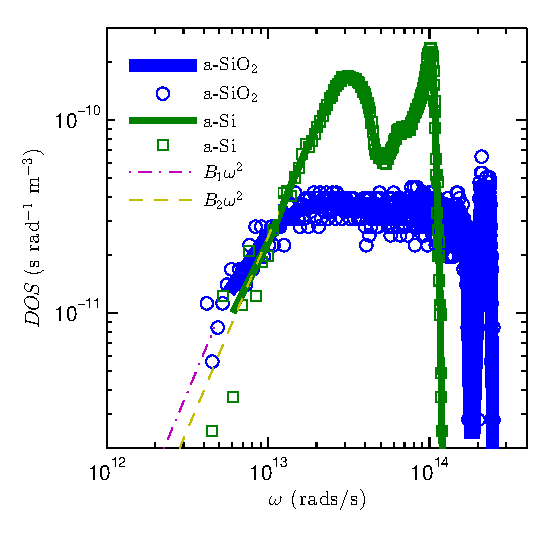
\includegraphics[scale=1.0]
{/home/jason/disorder/si/amor/m_af_si_normand_4096_DOS.eps}
\vspace*{-5mm}
\end{center}
\caption{\label{FIG:DOS} film thickness dependant thermal 
conductivity of a-Si from experiment.}
\end{figure}
%--------------------------------------------------------------------------
%\clearpage
%\vspace{50mm}

%--------------------------------------------------------------------------
\subsection{\label{S:Structure}Group Velocity}
%--------------------------------------------------------------------------

For a disordered solid, the three acoustic group 
velocities (two transverse and one 
longitudinal) can be predicted using the elastic constants
\cite{gale_general_2003} 
or by finite differencing of the three lowest frequency branches 
of the dispersion relation of the supercell.
\cite{feldman_thermal_1993,feldman_numerical_1999,
donadio_atomistic_2009,he_thermal_2011,
he_heat_2011,hori_phonon_2013,larkin_predicting_2013} 
Except for this low-frequency behavior, there is not an 
accepted method to predict the group velocity of a 
vibrational mode in a disordered system, although there have been 
attempts.
\cite{cahill_lattice_1988,duda_reducing_2011,donadio_atomistic_2009,
he_heat_2011,he_thermal_2011} 
In the Cahill-Pohl (CP) model, for example, the group velocity of 
all disordered modes is the sound speed, $v_s$, which is also assumed  
for the HS model, Eq. \eqref{EQ:M:k_AF,HS}.
\cite{cahill_lattice_1988} This assumption is not generally valid  
for any material.\cite{feldman_numerical_1999,duda_reducing_2011,
donadio_atomistic_2009,he_heat_2011,he_thermal_2011,larkin_predicting_2013}

Experimentally determined values
Freeman gives 4100 m/s for a-SiO$_2$\cite{freeman_thermal_1986}
3,700 5,100 from \cite{pohl_low-temperature_2002}
for a-Si 3,800-4,800\cite{pohl_low-temperature_2002}
Experimentally measured values of sound speed for a-Si are 4,160
\cite{senn_physics_1979} and 
4,290 m/s\cite{vacher_attenuation_1980}.
\cite{feldman_elastic_1991} 
For chemical vapor depositioned a-Si thin films, the transverse 
sound speed is markedly increased $v_{s,T} = 4,740$ m/s.
\cite{liu_high_2009} 


%--------------------------------------------------------------------------
\subsubsection{\label{S:Structure}From Elastic Constants and DOS}
%--------------------------------------------------------------------------

The transverse and logitudinal sound speeds of a material can be related 
to the material's elastic constants, which determine the bulk ($G$) and 
shear ($K$) moduli.(cite) The transverse sound speed is given by(cite)  
\begin{equation}\label{EQ:Dynamical}
v_{s,T} = \frac{G}{\rho}^{1/2},
\end{equation}
and the longitudinal by
\begin{equation}\label{EQ:Dynamical}
v_{s,L} = \frac{4G + 3K}{3\rho}^{1/2}.
\end{equation}
We use the bulk and shear moduli defined in terms of the elastic 
constants according to the Voight convention.(cite) 
The sound speeds calculated from the 
elastic constants are reported in Table . It is clear that the DOS of 
our models for a-Si and a-SiO$_2$ are characterized by using the 
transverse sound speeds, rather than an averaging of the transverse 
and longitudinal, 
\begin{equation}\label{EQ:Dynamical}
v_{s} = \frac{1}{3}v_{s,L} + \frac{1}{3}v_{s,T}. 
\end{equation}
This is backed up by theoretical(cite) and experimental(cite) results. 

%--------------------------------------------------------------------------
\subsubsection{\label{S:Structure}From Struture Factor}
%--------------------------------------------------------------------------

Calculating the structure factors of the supercell Gamma   
modes is a method to test for their plane-wave 
character at a particular wave vector and 
polarization corresponding to the VC. 
\cite{allen_diffusons_1999,feldman_numerical_1999} 
Feldman et al. used the structure factor to predict an effective 
dispersion for a model of amorphous silicon, but did not predict 
group velocities.\cite{feldman_numerical_1999} 
Volz and Chen used the dynamic structure factor to predict the
dispersion of crystalline SW silicon using MD simulation.
\cite{volz_molecular-dynamics_2000} Has also been used to determine 
the dispersion relation from experimentally derived predictions.
\cite{green_density_2011} 

The structure factor at a VC wave vector 
$\pmb{\kappa}_{VC}$ is defined as\cite{allen_diffusons_1999} 
\begin{equation}\label{EQ:SLT}
S^{L,T}\kvcw = 
\sum_{\nu} E^{L,T}\kvcv
\delta [\omega-\omega\kgv],
\end{equation}
where the summation is over the Gamma modes, $E^{T}$ refers 
to the transverse polarization and is defined as
\begin{equation}\label{EQ:EL}
E^L\kvcv = 
\left|
\sum_{b} 
\hat{\pmb{\kappa}}_{VC} \cdot e\kgvba 
\EXP{i\pmb{\kappa}_{VC}\cdot\pmb{r}_0\ab{l=0}{b}} 
\right|^2
\end{equation}
and $E^{L}$ refers to the longitudinal polarization and is defined as
\begin{equation}\label{EQ:ET}
E^T\kvcv = 
\left|
\sum_{b} 
\hat{\pmb{\kappa}}_{VC} \times e\kgvba 
\EXP{i\pmb{\kappa}_{VC}\cdot\pmb{r}_0\ab{l=0}{b}} 
\right|^2.
\end{equation}
In Eqs. \eqref{EQ:EL} and \eqref{EQ:ET}, the $b$ summations are 
over the atoms in the disordered supercell, 
$\pmb{r}_0\ab{l=0}{b}$ refers to the equilibrium atomic position of 
atom $b$ in the supercell, $l$ labels the unit cells 
($l=0$ for the supercell), 
$\alpha$ labels the Cartesian coordinates, and 
$\hat{\pmb{\kappa}}_{VC}$ is a unit vector.  
Explicit disorder is included in the Gamma frequencies 
$\omega\kgv$ and the $3N_a$ components of the eigenvectors, $e\kgvba$.

The structure factors $S^{L,T}(\kappa,\omega)$ are plotted in Fig. for 
a-SiO$_2$ and a-Si (left and right panels) for wavevectors along the 
[100] direction of the 
supercells. The length scale used for the wavevectors, $\kappa = 2\pi/a[100]$,
are $a = $ 4.8 and 5.43 $\AA$ for a-SiO$_2$ and a-Si, which are based 
on the atomic number densities.(cite) 
Frequencies $\omega_0(\kappa)$ and lifetimes $\Gamma(\kappa)$ are predicted 
by fitting each structure 
factor peak $S^{L,T}\kvcw$ to a Lorentzian function
\begin{equation}\label{EQ:Lorentzian_NMD}
\begin{split}
S^{L,T}(\kappa,\omega) = \sum_{\nu}^{3n}
\frac{C_0(\nu)}{[\omega_0(\kappa)-\omega]^2+\Gamma^2(\kappa)},
\end{split}
\end{equation}
where $C_0(\nu)$ is a constant related to the DOS.
\cite{beltukov_ioffe-regel_2013} A dispersion relation is identified by 
plotting $\omega_0(\kappa)$ in the middle panel of Fig. , where the bars 
indicate the peak widths $\Gamma(\kappa)$. 

Sound speeds are estimated by finite differencing, 
\begin{equation}\label{EQ:Dynamical}
\pmb{\text{v}_{s}} = \frac{ \delta \omega_0(\kappa)}{\delta \kappa}.
\end{equation}
Estimates of the sound speeds are found from using finite difference 
of the peaks in $S_{T,L}$ are shown in Table. The values are close to 
those obtained from the elastic constants (see Section ). 

The dispersion for a-SiO$_2$ 
The dispersion for a-SiO$_2$ more closely resembles the so-called 
''dispersion law for diffusons``, where $\omega \propto q^2$.
\cite{beltukov_ioffe-regel_2013}

The structure factor gives the frequency spectrum
needed to construct a (nonstationary) propagating state with a
pure wave vector Q and pure longitudinal or transverse polarization
 \cite{feldman_thermal_1993}. Only low-frequency vibrations 
have an (approximate) wavevector in disordered systems, and there is 
no theorem guranteeing this. \cite{feldman_numerical_1999}
you cannot assign a unique wavevector to individual modes, 
even for low frequency modes.
\cite{biswas_vibrational_1988,feldman_thermal_1993,silbert_normal_2009}

Fig 4 of this work shows a dispersion extracted by locating the peaks in 
the structure factor. The dispersion at low 
frequency is also dominated by transverse sound speed.\cite{vitelli_heat_2010} 

The transverse sound speed predicted by the DOS is used for both 
a-SiO$_2$ and a-Si throuhout the rest of this work. 

%--------------------------------------------------------------------------
\begin{figure}
\begin{center}
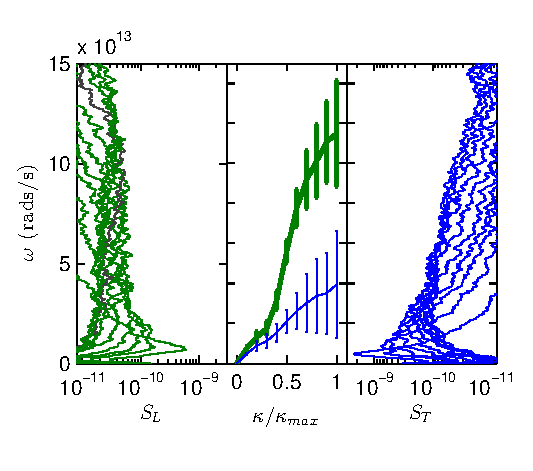
\includegraphics[scale=1.0]
{/home/jason/disorder/si/amor/m_af_si_normand_4096_disp_sio2_2.eps}
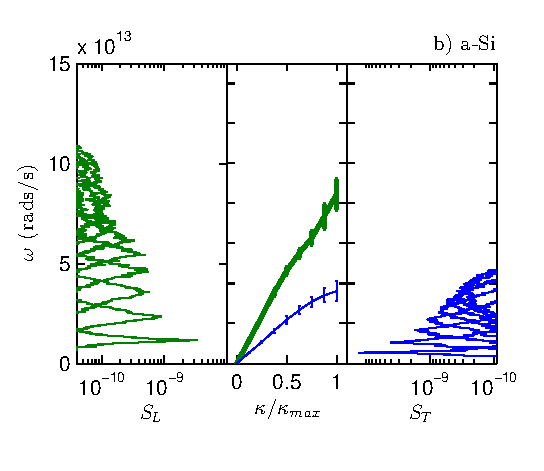
\includegraphics[scale=1.0]
{/home/jason/disorder/si/amor/m_af_si_normand_4096_disp_si.eps}
\end{center}
\caption{\label{FIG:disp} film thickness dependant thermal 
conductivity of a-Si from experiment.}
\end{figure}
%--------------------------------------------------------------------------

%--------------------------------------------------------------------------
\begin{center}
%\begingroup
\squeezetable
\begin{table}
\caption{\label{T:vs}
Estimated from the elastic constants, the pre-annealed group velocities are 
$v_{s,T,} = 3,670$ , $v_{s,L,elas} = 7,840$
$v_{s,T,elas} = 2,541$ , $v_{s,L,elas} = 4,761 $ (see Section ).
}
\begin{ruledtabular}
\begin{tabular}{llllll}
\hline
method~~~~~~~\vline $B_{mod}$ (Eq. \eqref{EQ:Bmod}) \vline $S_{T,L}$ (Eq. \eqref{EQ:SLT}, \eqref{EQ:dwdk} )  \vline DOS (Eq. \eqref{EQ:DOS_debye})  \\
\hline
a-SiO$_2$  \\
\hline
transverse~~~~\vline 3,161~~~~~~~~~~~~~~~ \vline 2,732~~~~~~~~~~~~~~~~~~~~~~ \vline 2,339  \\
\hline
longitudinal~\,\vline 5,100~~~~~~~~~~~~~~~ \vline 4,779~~~~~~~~~~~~~~~~~~~~~~ \vline   \\
\hline
a-Si  \\
\hline
transverse~~~~\vline 3,886~~~~~~~~~~~~~~~ \vline 3,699~~~~~~~~~~~~~~~~~~~~~~ \vline 3,615  \\
\hline
longitudinal~\,\vline 8,271~~~~~~~~~~~~~~~ \vline 8,047~~~~~~~~~~~~~~~~~~~~~~ \vline   \\
\end{tabular}
\end{ruledtabular}
\end{table}
%\endgroup
\end{center}
%--------------------------------------------------------------------------

%\clearpage
%\vspace{50mm}

%--------------------------------------------------------------------------
\subsection{\label{S:Life}Mode Lifetimes}
%--------------------------------------------------------------------------

In conclusion, we have found that the high-frequency
VS in a realistic model of amorphous Si decay on picosec-
ond time scales, and at low temperatures their lifetimes de-
crease as frequency increases. This is in contrast to recent
experimental claims that the modes decay on nanosecond
scales and their lifetimes increase as frequency increases.
\cite{fabian_anharmonic_1996} 

The lifetimes found by this method
are in good agreement with the perturbative calculations of
Fabian and Allen and are on the order of 10 ps at low tem-
peratures in both 216 and 4096 atom supercells.
\cite{bickham_calculation_1998}

Our results indicate that all of
these processes occur on a much faster time scale than the
ϳ1 ns temporal resultion of the Raman experiments, so it is
not obvious that the measured relaxation rates should be
identified with vibrational lifetimes.
\cite{bickham_numerical_1999}


%--------------------------------------------------------------------------
\subsubsection{\label{S:Life_SF}From Structure Factor}
%--------------------------------------------------------------------------

The lifetimes predicted from Eq. are plotted in Fig. for a-SiO2 and a-Si. 
There is a clear separation for transverse and longitudinal scalings 
for a-Si with $tau \propto \omega^{-2}$, and the lifetimes are above the 
IR limit (Eq. ) for the lowest frequencies. 

For a-SiO2, the separation between transverse and longitudinal is not 
as clear as in a-Si, and the lifetimes are significantly less than the 
IR limit, Eq. .  

Ioffe-Regel limit \cite{taraskin_determination_1999}.

%--------------------------------------------------------------------------
\begin{figure}
\begin{center}
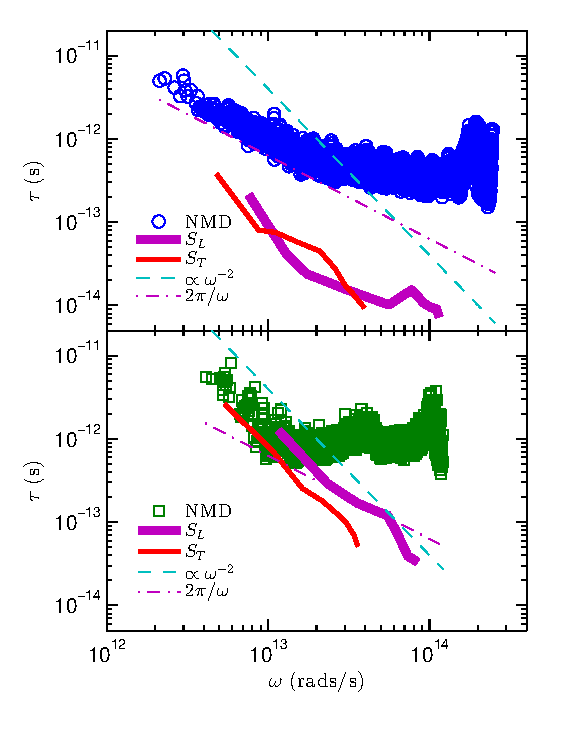
\includegraphics[scale=1.0]
{/home/jason/disorder/si/amor/m_af_si_normand_4096_tau_2.eps}
\vspace*{-5mm}
\end{center}
\caption{\label{FIG:Lifetimes} film thickness dependant thermal 
conductivity of a-Si from experiment.}
\end{figure}
%--------------------------------------------------------------------------

%--------------------------------------------------------------------------
\subsubsection{\label{S:Life_NMD}From Normal Mode Decomposition}
%--------------------------------------------------------------------------

We use the MD simulation-based 
normal mode decomposition (NMD) method to predict the lifetimes of each 
vibrational mode in the disordered supercells (see Section ).
\cite{ladd_lattice_1986,mcgaughey_quantitative_2004,
turney_predicting_2009-1,larkin_comparison_2012} 
The NMD method can predict vibrational lifetimes which are affected by 
the disorder in the supercell.(cite) 

(footnote)
In NMD, the 
atomic trajectories from MD simulations are first mapped onto the vibrational 
mode coordinate time derivative,
\cite{dove_introduction_1993}
\begin{equation}\label{EQ:qdot}
\begin{split}
\dot{q}\kvt{}{}{}=&\SUM{0}{}\sqrt{\frac{m_b}{N}}\dot{u}_{\alpha}
\lbt e^*\kvba\EXP{i\pmb{\kappa}\cdot\mathbf{r}_0\ab{l}{0}}.
\end{split}
\end{equation}
Here, $m_b$ is the mass of the $b_{th}$ atom in the unit cell, 
$u_{\alpha}$ is the $\alpha$-component of the atomic displacement 
from equilibrium, $\dot{u}_{\alpha}$ is the $\alpha$-component 
of the atomic velocity, and $t$ is time.    
The spectral energy of each vibrational mode, $\Phi\kvt$, is calculated 
from 
\begin{equation}\label{A:E:Lorentzian_NMD}
\begin{split}
\Phi(\pmb{\kappa},\omega) = 2\sum_{\nu}^{3n} T\kvw=2\sum_{\nu}^{3n} 
\lim_{\tau_0\rightarrow\infty}\frac{1}{2\tau_0}
\left|\frac{1}{\sqrt{2\pi}}\int_{0}^{\tau_0}\dot{q}\kvt
\exp(-i\omega t)dt\right|^2,
\end{split}
\end{equation}

The vibrational mode frequency and lifetime is predicted by fitting each mode's 
spectral energy $\Phi(\nu,\omega)$ (see Appendix ) to a Lorentzian function
\begin{equation}\label{EQ:Lorentzian_NMD}
\begin{split}
\Phi(\nu,\omega) = \sum_{\nu}^{3n}
\frac{C_0(\nu)}{[\omega_0(\nu)-\omega]^2+\Gamma^2(\nu)},
\end{split}
\end{equation}
where the constant $C_0(\nu)$ is related to the average energy of 
each mode and the linewidth $\Gamma(\nu)$.
\cite{larkin_comparison_2012} The mode lifetime is given by
\begin{equation}\label{EQ:Life}
\begin{split}
\tau(\nu) = \frac{1}{2\Gamma(\nu)}
\end{split}
\end{equation}

For a-SiO2, the mode lifetimes are generally larger than the 
IR limit Eq. , and follow this limit at low frequency. 
At high frequency the mode lifetimes are roughly constant 
without definite scaling. There is a peak near 
2 10^{14} rads/s which corresponds to a peak in the DOS (see Fig. ).  

The mode lifetimes show a similar 
plateau at higher frequencies, particularly for a-Si, which has been 
reported for disordered lattices.\cite{larkin_predicting_2013}

For a-Si, a transition to a constant lifetime plateau occurs near 
1 10^{14} rads/s, which corresponds to where the DOS peaks in Fig. . 
Similar behavior was observed for model disordered lattices.
\cite{he_heat_2011,larkin_predicting_2013} 



%--------------------------------------------------------------------
%\begin{figure}
%\begin{center}
%\includegraphics[scale=1.0]
%{/home/jason/disorder/si/amor/m_si_amor_life_he_compare.eps}
%\vspace*{-5mm}
%\end{center}
%\caption{\label{FIG:phonon_diff} film thickness dependant thermal 
%conductivity of a-Si from experiment.}
%\end{figure}
%--------------------------------------------------------------------------

%\clearpage
%\vspace{50mm}

%--------------------------------------------------------------------------
\subsubsection{\label{S:Life_NMD}Discussion}
%--------------------------------------------------------------------------


These time scales are close to those reported in Ref for similar 
a-Si structures. The lifetimes are also on the order of those
reported for similar models of a-Si using MD-based and anharmonic 
lattice dynamics methods.(cite) 

A previous study of a-Si predicted vibrational lifetimes on the 
order of 100 ps, about ten times the values reported here and in 
other studies.(cite) While the samples 

For a-Si, the scaling at low frequency shows 
$\tau \propto \omega^{-2}$.  The same scaling was found in previous 
studies using similar models for a-Si.(cite) 

Also
shown as a solid curve is the phonon gas model, where the
fitted formula 1/␶ Q ϭ2⌫ i κQ 2
is used for transverse
i
propagons, and it is assumed that transverse and longitudinal
propagons have the same diffusivity. Notice that the gas-
model result fits perfectly onto the higher frequency diffuson
result, indicating mutual consistency of the two different
transport theories in the region of overlap 10 meV Ͻ␻Ͻ20
meV.

%--------------------------------------------------------------------------
\subsection{\label{S:Diffusivities}Diffusivities}
%--------------------------------------------------------------------------


Thermal diffusivity was predicted for a percolation network which showed 
Rayleigh type scattering dependance in the low-frequency limit.
\cite{sheng_heat_1991}

which generally agree with diffusivities computed according to the 
formula of Edwards and THoules.\cite{edwards_numerical_1972,
feldman_numerical_1999,beltukov_ioffe-regel_2013}

Thermal diffusivity has been predicted using a wave-packet method

It was shown 

Garber shows that these high-frequency modes are localized in the 
Anderson sense, showing exponential decay of the mode eigenvector.
\cite{garber_numerical_2001}

It was shown that the diffusivity $D_{AF}(\omega) \propto DOS(\omega)$ 
at low frequency when the modes are spatially uncorrelated and the 
overlap between them is small and independent of the frequency.
\cite{vitelli_heat_2010,xu_energy_2009}

At low frequencies, the AF-predicted and NMD-predicted mode 
diffusivities scale as $D \propto \omega^{-2}$, similar to the scaling 
due to Umklapp scattering of phonons in a crystalline system. Rayleigh 
scattering due to point defects predicts $D \propto \omega^{-4}$, 
but is not observed in the amorphous systems studied in this work.(cite) 
While Rayleigh-type scaling has been 
observed in harmonic studies of the diffusivities of modes in 
disordered lattics and jammed systems,
\cite{sheng_heat_1991,xu_energy_2009,vitelli_heat_2010} 
it has been demonstrated that the harmonic disorder in a-Si 
produces a scaling similar to Umklapp scattering.
\cite{feldman_thermal_1993}

In summary, we obtain a frequency-independent diffusiv-
ity when the density of states is frequency-independent and
the following conditions are satisfied: ͑A͒ displacements of
particles in different modes of similar frequency are uncor-
related; ͑B͒ the directions of changes in the relative displace-
ments of pairs of interacting particles are spatially uncorre-
lated within a given mode; and ͑C͒ the direction of change in
the relative displacement of a pair of interacting particles is
uncorrelated from the direction of the displacement.

Both a-SiO$_2$ and a-Si have a region at higher frequencies where the 
AF-predicted mode diffusivities are relatively constant. This behavior 
has been reported for a number of disordered systems such as 
disordered lattices
\cite{sheng_heat_1991,beltukov_ioffe-regel_2013,larkin_predicting_2013} 
and jammed systems. At the higest frequencies the AF-predicted 
diffusivities trend exponentially to zero, which is an indication 
that these modes are ''locons``, spatially localized modes which 
do not contribute to thermal condutivity.\cite{allen_diffusons_1999} 

This perplexing property of glasses
has been explained heuristically by assuming that phonons
are scattered so strongly by structural disorder that trans-
port becomes diffusive, with a frequency regime of small,
constant thermal diffusivity.
\cite{kittel_interpretation_1949,sheng_heat_1991,allen_} 

%--------------------------------------------------------------------------
\subsection{\label{S:Diffusivities}Discussion}
%--------------------------------------------------------------------------

This supports the idea of Slack for a-SiO$_2$\cite{slack_thermal_1979}
While the thermal conductivity of a-SiO , the material is characterized by 
a constant similar for other amorphous
materials such as Lennard-Jones argon\cite{larkin_predicting_2013} 
and a model of a-GeTe.\cite{sosso_thermal_2012}

At low frequency, our model supports the scaling 
$D(\omega) = B \omega^{-2}$ and not $D(\omega) = B \omega^{-4}$ as is 
predicted by the Rayleigh scattering from density fluctuations acting 
as scattering centers.(cite) Rayleigh scattering 


%--------------------------------------------------------------------------
\begin{figure}
\begin{center}
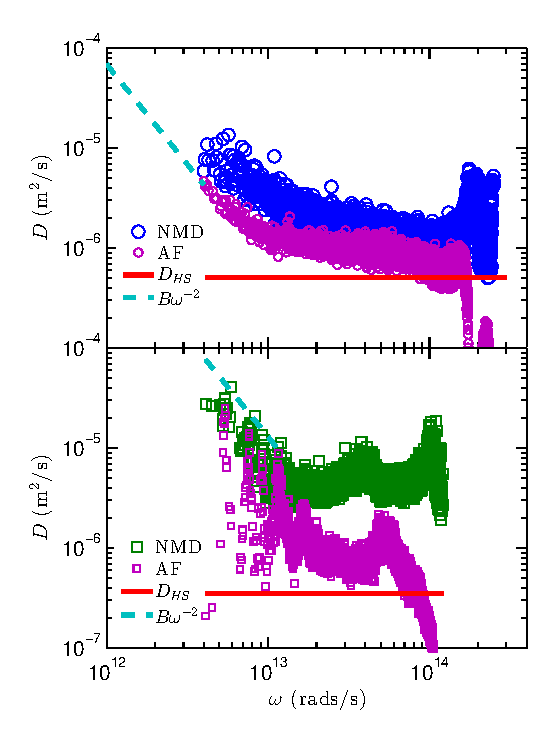
\includegraphics[scale=1.0]
{/home/jason/disorder/si/amor/m_af_si_normand_4096_D_2.eps}
\vspace*{-5mm}
\end{center}
\caption{\label{FIG:diffusivities} film thickness dependant thermal 
conductivity of a-Si from experiment.}
\end{figure}
%--------------------------------------------------------------------------

\begin{equation}\label{EQ:Life}
\begin{split}
v_{AF} = \frac{D_{i}}{2\Gamma(\nu)}
\end{split}
\end{equation}

%--------------------------------------------------------------------------
\begin{figure}
\begin{center}
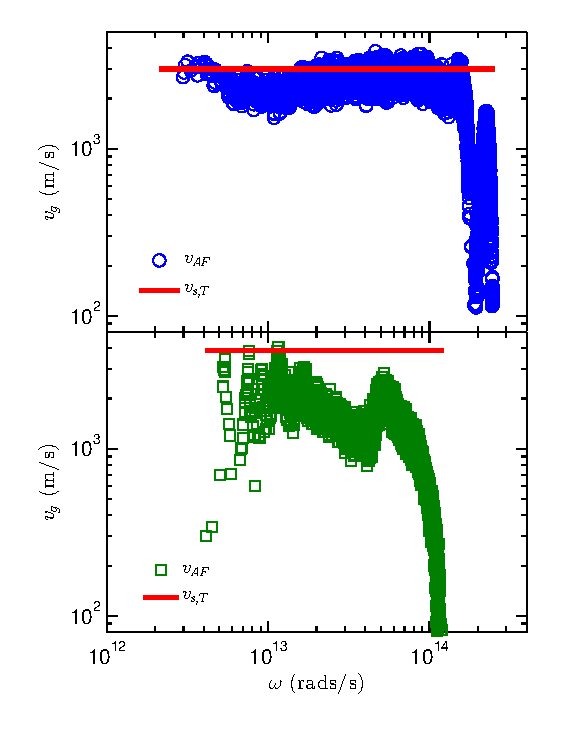
\includegraphics[scale=1.0]
{/home/jason/disorder/si/amor/m_af_si_normand_4096_vAF.eps}
\vspace*{-5mm}
\end{center}
\caption{\label{FIG:Lifetimes} .}
\end{figure}
%--------------------------------------------------------------------------


%\clearpage
%\vspace{50mm}

%--------------------------------------------------------------------------
\subsection{\label{S:MFP}Mean Free Paths}
%--------------------------------------------------------------------------

Using the lifetimes predicted from the structure factor peaks and the 
transverse sound speed, the MFP is about the size of the simulation cell 
$L$. 



%--------------------------------------------------------------------------
\begin{figure}
\begin{center}
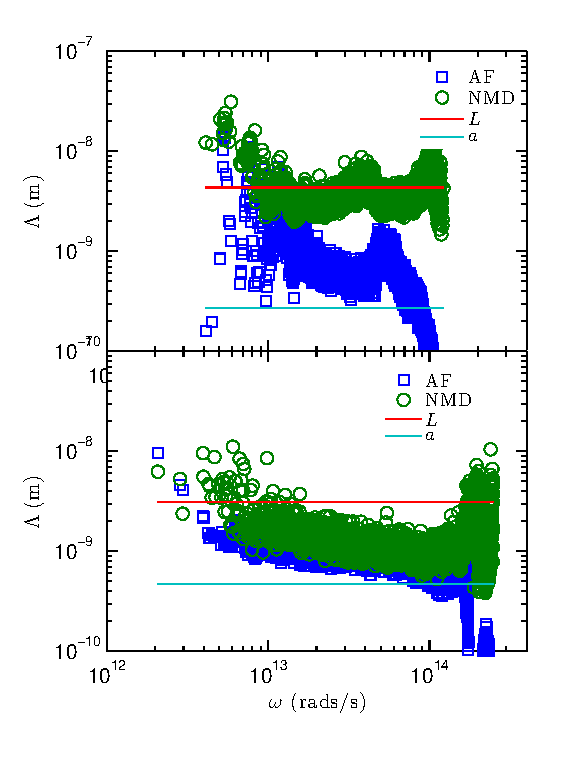
\includegraphics[scale=1.0]
{/home/jason/disorder/si/amor/m_af_si_normand_4096_Lambda.eps}
\vspace*{-5mm}
\end{center}
\caption{\label{FIG:mfp} film thickness dependant thermal 
conductivity of a-Si from experiment.}
\end{figure}
%--------------------------------------------------------------------------

%\clearpage
%\vspace{50mm}

%--------------------------------------------------------------------------
\section{\label{S:Conductivity}Thermal Conductivity}
%--------------------------------------------------------------------------

%--------------------------------------------------------------------------
\subsection{\label{S:Bulk}Bulk}
%--------------------------------------------------------------------------

Lee found a value of around 1 W/m-K 
but with very small supercell sizes.\cite{lee_molecular-dynamics_1991}

We use the GK method to predict the thermal conductivity. The GK method 
is relatively inexpensive compared to the NMD and AF methods so that 
large system sizes 
can be simulated (see Section ).  

For smaller system sizes, the same trajectories are used for the GK and 
NMD methods. The MD simulations were run with the same parameters 
as the NMD metho (see Section ). 

The predicted thermal condcutivties from the GK method are plotted 
in Fig. . For a-SiO2, the thermal conductivity is size independent 
within the errors.  For a-Si, there is a clear size-dependance of the 
thermal conductivity

To compare the results of the mode-based methods (NMD and AF) and 
the GK method, it is necessary to estimate the missing contribution from 
vibrational modes with frequency less than the minimum frequency of 
the finnite systems. 

Assuming the thermal conductivity form Eq.  for the lowest frequency modes in 
the system, the thermal conductivity as a function of the system size 
takes the form
\begin{equation}\label{EQ:k0}
\frac{k(N_0)}{k_{bulk}} = 1 - \frac{c_0}{N_0},
\end{equation}

``We find that we cannot define a wave vector for the
majority of the states, but the intrinsic harmonic diffusivity is still well-defined and has a numerical value
similar to what one gets by using the Boltzmann result, replacing v by a sound velocity and replacing l by
an interatomic distance a.
''\cite{feldman_thermal_1993}

``In order to fit the experimental sc( T) it is necessary to add a Debye-
like continuation from 10 meV down to 0 meV. The harmonic diffusivity becomes a Rayleigh m
law
and gives a divergent ~(T) as T~O. To eliminate this we make the standard assumption of resonant-
plus-relaxational absorption from two-level systems (this is an anharmonic effect which would lie outside
our model even if it did contain two-level systems implicitly).
''\cite{feldman_thermal_1993}



Debye model. k_tot = k_phonon + k_AF. For lack of a rigorous definition 
of phonon vs diffusion, we will define k_phon = k_debye. 

The relative contribution of k_phonon and k_AF is also predicted to 
be similar for silicon nanowires.\cite{donadio_atomistic_2009} 

%--------------------------------------------------------------------------
\begin{figure}
\begin{center}
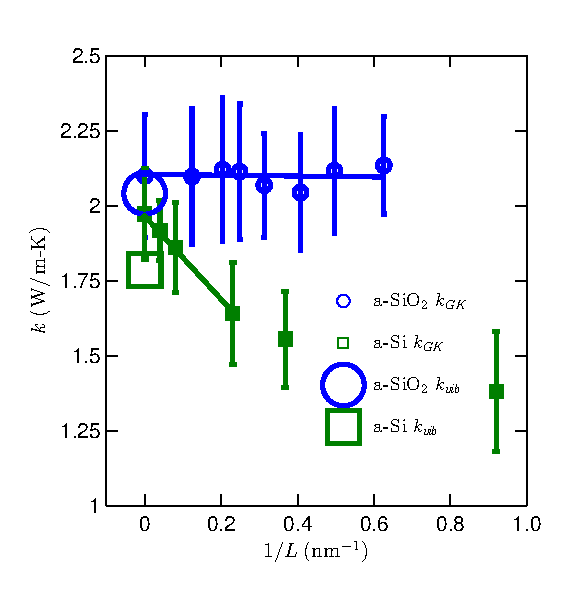
\includegraphics[scale=1.0]
{/home/jason/disorder/si/amor/m_af_si_normand_4096_gk_cond_2.eps}
\vspace*{-5mm}
\end{center}
\caption{\label{FIG:cond} Thermal conductivities of a-SiO^2 and 
a-Si prediced using the GK method.}
\end{figure}
%--------------------------------------------------------------------------

%--------------------------------------------------------------------------
\subsection{\label{S:Accumulation}Accumulation}
%--------------------------------------------------------------------------

%--------------------------------------------------------------------------
\begin{figure}
\begin{center}
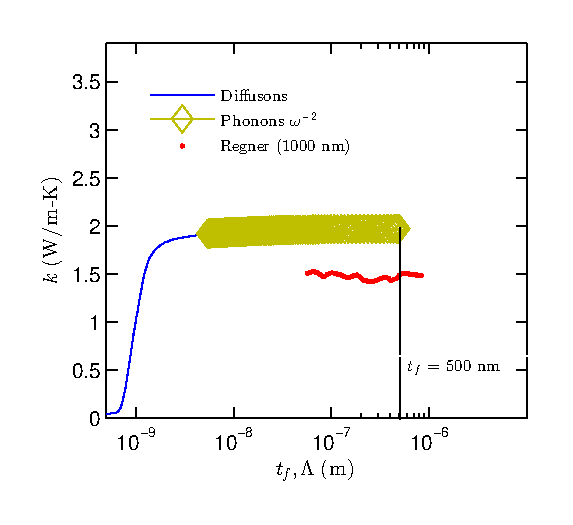
\includegraphics[scale=1.0]
{/home/jason/disorder/si/amor/m_af_si_normand_4096_kLamba_4_sio2.eps}
\vspace*{-5mm}
\end{center}
\caption{\label{FIG:accum} film thickness dependant thermal 
conductivity of a-Si from experiment.}
\end{figure}
%--------------------------------------------------------------------------

%--------------------------------------------------------------------------
\begin{figure}
\begin{center}
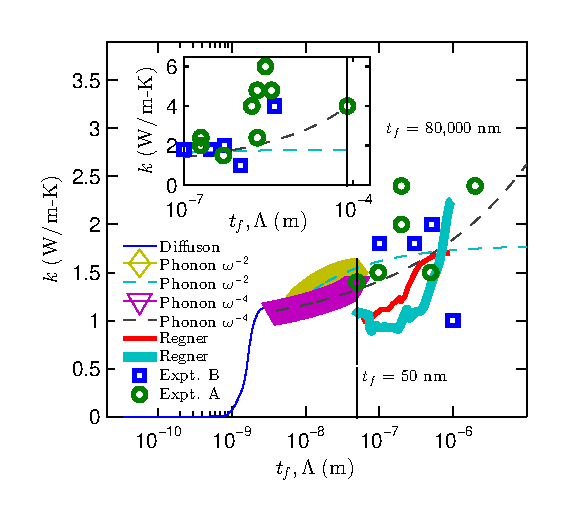
\includegraphics[scale=1.0]
{/home/jason/disorder/si/amor/m_af_si_normand_4096_kLamba_4_si.eps}
\vspace*{-5mm}
\end{center}
\caption{\label{FIG:accum} film thickness dependant thermal 
conductivity of a-Si from experiment.}
\end{figure}
%--------------------------------------------------------------------------

%\clearpage
%\vspace{50mm}

%--------------------------------------------------------------------------
\subsection{\label{S:Lifetimes}Discussion}
%--------------------------------------------------------------------------

This agress with previous estimates for the contribution of low 
frequency ($\omega<30 rads/s$) \cite{love_estimate_1990}

Moedling shows that alloying a-Si with Ge can further reduce 
the thermal conductivity of the bulk and thin films.
\cite{bouchard_vibrational_1988,feldman_thermal_1993} 

scattering from static imperfections would predicts Rayleigh type 
scattering \cite{klemens_scattering_1955}
what if you choose a rayleigh type model with 
``To implement Eq. ͑6͒ one must know the
correct Q dependence of ⌫ Q . As shown in Fig. 8, the fitted
values scatter too much to guide the extrapolation well. In
principle, at very small Q one should get a form ⌫ Q ϭCQ 4
which corresponds to Rayleigh scattering of sound waves
from the structural disorder. The data of Fig. 8 do not fit a
Q 4 law; the Q 2 curve shown in the figure is a better fit. Two
experiments13,15 ͑but not a third35͒ and one calculation18 on
a-SiO2 have also given ⌫κQ 2 . We do not know a theory
which can give this law in a harmonic model.

The agree-
ment between the 3! and the TDTR measurements at
1.11 MHz suggests that phonons with ‘ > ðD=!Þ1=2 1⁄4
612 nm are not significant for thermal conduction in this
sample. Furthermore, the difference between the high and
low frequency measurements by TDTR indicates that pho-
nons with 162 < ‘ < 612 nm contribute 40$\%$ of the of
the sample.\cite{liu_high_2009}

The acoustic projected spectral density SðQ; EÞ is shown
in Fig. 3. From the Q 1⁄4 h100i transverse and longitudinal
projections, we obtain the respective phase velocities of
vt = 4,740 $v_l$ = 7,830 m/s Wooten model, where $v_t$ is 
significantly higher than the value for our a-Si model 
(see Table ).\cite{liu_high_2009} 

Even though the DOS of the WWW produced structures compare well with 
other models and also experimental measurements, it has been 
demonstrated that the spectral properties at low frequency can be 
much different, particularly the linewdith of the structure 
factor.\cite{liu_high_2009} It is possible that the 

Based on the variation of thermal conductivity with film thickness, 
Liu et al also report a MFP scaling of 
$\Lambda \propto \omega^{-2}$.\cite{liu_high_2009} Similar experimental 
results were obtained for a-SiO$_2$.
\cite{masciovecchio_evidence_2006}

Tight-binding models for a-Si can improve the low-frequency 
DOS prediction compared to experiment.\cite{feldman_tight-binding_2004}


A combination of frequency-domain, time-domain, and variable 
physical heating size measurments would be helpful in investigating
\cite{koh_frequency_2007,siemens_quasi-ballistic_2010,
minnich_thermal_2011,regner_broadband_2013}


%--------------------------------------------------------------------------
\section{\label{S:Lifetimes}Summary}
%--------------------------------------------------------------------------

Table \ref{T:cond_table}.

%--------------------------------------------------------------------------
% \begin{center}
% %\begingroup
% %\squeezetable
% \begin{table}
% \caption{\label{T:cond_table}Thermal conductivity predictions using the 
% VC-NMD, VC-ALD, and GK methods. For LJ argon alloys, the bulk extrapolation 
% is used for all three methods.  For SW silicon alloys, only VC-ALD and GK 
% can be used to extrapolate a bulk thermal conductivity 
% (see Section \ref{S:Thermal Conductivity}). For VC-NMD and GK, the 
% uncertainties 
% are estimated by omitting independent simulations from 
% the ensemble averaging (see Section \ref{S:Calculation}). For VC-ALD, 
% the uncertainties are estimated by omitting extrapolation points used for 
% Eq. \eqref{EQ:k0}.}
% \begin{ruledtabular}
% \begin{tabular}{llllll}
% $c$  ~~~~\vline GK ~~~~~~~~~~~ \vline VC-NMD~~~~\, \vline VC-ALD~~~~~\, \vline VC-NMD$^*$~~~ \vline VC-ALD$^*$ ~~\: \vline  \\
% \hline
% LJ  \\
% \hline
% 0.00 \vline 3.3 $\pm$ 0.1 ~~~\, \vline 3.3 $\pm$ 0.1 ~~ \,\, \vline 3.4 $\pm$ 0.1 ~~~\,\,\, \vline ~~~~~~~~~~~~~~\;~\,\, \vline~~~~~~~~~~~~~\:\:\,\, ~ \vline \\
% 0.05 \vline 0.80 $\pm$ 0.07 \, \vline 0.76 $\pm$ 0.07 ~ \vline 0.45 $\pm$ 0.02 ~\, \vline 0.80 $\pm$ 0.1 \,  ~ \vline 0.52 $\pm$ 0.05  ~ \vline  \\
% \end{tabular}
% \end{ruledtabular}
% \end{table}
% %\endgroup
% \end{center}
%--------------------------------------------------------------------------

% %--------------------------------------------------------------------------
% \begin{figure}
% \begin{center}
% \includegraphics[scale=0.6]
% {/home/jason/disorder/matlab/galli_si_k_tf.eps}
% \vspace*{-5mm}
% \end{center}
% \caption{\label{FIG:phonon_diff} film thickness dependant thermal 
% conductivity of a-Si from experiment.}
% \end{figure}
% %--------------------------------------------------------------------------

\clearpage
\bibliographystyle{apsrev}
\bibliography{/home/jason/Dropbox/ntpl-paper/ntpl-060313}
\end{document}
% 